\documentclass[a4paper,11=0pt]{article}
\usepackage[margin=1.15in, top=1.15in,bottom=1.15in]{geometry}
\usepackage{amsmath}
\usepackage{gensymb}
\usepackage{graphicx}
\usepackage{mathtools}
\usepackage{booktabs}
\usepackage{multirow}
\usepackage{mathtools}
\usepackage{caption}
\usepackage{parskip}
\usepackage{tikz}
\usepackage{csquotes}
\usepackage{hyperref}
\renewcommand\rmdefault{ptm} % use Times
\let\boldtheta\theta % make theta into vector
\renewcommand{\theta}{\boldsymbol{\boldtheta}} % make theta into vector
\renewcommand{\d}{\: \mathrm{d}} % fix d in integrals
\usepackage{scrextend} % for lists

\title{\vspace*{-1.5em}\textbf{Project Proposal}\\ \vspace{0.25em} \Large Investigating Bayesian Inference in Continual Learning}

\author{M. E. Tong, supervised by S. Farquhar and Y. Gal}

\date{}

\begin{document}

\maketitle

%Background: the theory or application areas;
%General open questions;
%Selection of particular question for study;
%Proposed method;
%Draft Timetable;
%Signature of Project Supervisor.

For real-world problems, it is vital that intelligent agents have the capacity to learn and remember a variety of tasks \cite{ewc}. Continual learning refers to online multi-task learning where tasks are learned sequentially, with datasets discarded after training. It is of particular importance for applications for which retaining old datasets is unethical, undesireable, illegal or imprudent \cite{unifying, robust}.

The major problem in the field is that of catastrophic forgetting. New learning often causes neural networks to rapidly forget old learning \cite{catastrophic}. The challenge is to balance learning new tasks whilst remembering previous ones. Though promising results have been published in the field of continual learning, clear shortcomings have been identified in many of the current approaches and evaluations, such as a dependency on re-training on previous datasets or tasks \cite{robust}. 

The most recent advances in continual learning have favoured a prior-focused approach, such as variational continual learning \cite{vcl}, synaptic intelligence \cite{si}, elastic weight consolidation \cite{ewc}, Riemannian walk \cite{rw} and Kronecker factored online Laplace approximation \cite{ritter}. These prior-focused approaches use the posterior or other parameters from previous tasks as priors for new tasks. Likelihood-based approaches, such as Deep Generative Replay \cite{dgr}, are based on pseudo-rehearsal \cite{robins}, simulating previous datasets in order to estimate their log-likelihood according to the new model. There have also been approaches based on dynamic architectures. %Rusu 2016, Li and Hoiem 2017

\vspace{-0.5em}
\subsubsection*{Variational Continual Learning}

\vspace{-1em}
We suggest that further investigation into the variational continual learning (VCL)  \cite{vcl} approach is warranted. Currently, good performance is dependent on re-training on small coresets retained from previous datasets \cite{robust}, but improvements to the approach may eliminate the need for these coresets, which would better reflect true continual learning.

VCL demonstrates a prior-focused Bayesian approach to continual learning, where the posterior for the previous tasks is used as the prior when training on the new task dataset. This is an intuitive way of allowing the previous tasks to strongly influence prediction, whilst allowing the parameters to adapt to the new task. 
\begin{equation}\label{eq:1}
\begin{split}
\underbrace{p(\theta | \mathcal{D}_{1:t})}_{\mathclap{\text{new posterior}}} \propto \underbrace{p(\theta | \mathcal{D}_{1:t-1})}_{\substack{\text{previous posterior}\\ (\text{new prior})}} \underbrace{p(\mathcal{D}_t | \theta)}_{\text{likelihood}}
\end{split}
\end{equation}


However, the true posterior $p(\theta | \mathcal{D}_{1:t})$ is computationally intractable, so we must approximate it. We suggest that improvements to this approximation may be key to performance. 


The posterior approximation in VCL is performed using Kullback-Leibler (KL) minimisation, a variational method, over a model family of possible posteriors $\mathcal{Q}$, to yield a tractable normalised approximation $q_t(\theta)$ to the true posterior $p(\theta | \mathcal{D}_{1:t})$. We define $q_0(\theta)$ to be the prior, $p(\theta)$.

\vspace{-1.7em}
\begin{equation}\label{eq:3}
\begin{split}
\underbrace{p(\theta | \mathcal{D}_{1:t})}_{\mathclap{\substack{\text{new true}\\ \text{posterior}}}}\approx \underbrace{q_t(\theta)}_{\mathclap{\substack{\text{new posterior}\\ \text{approximation}}}} &=\underset{q\in\mathcal{Q}}{\mathrm{arg}\mathrm{min}} \: \mathrm{KL}\bigg(q(\theta)\:||\:\frac{1}{Z_t}\underbrace{q_{t-1}(\theta)}_{\mathclap{\substack{\text{previous posterior} \\ \text{approximation}}}}p(\mathcal{D}_t|\theta) \bigg)\\
\end{split}
\end{equation}
Here, $\theta$ are the parameters, $\mathcal{D}_i$ is the $i$\textsuperscript{th} dataset, $q_i(\theta)$ is the posterior approximation following the $i$\textsuperscript{th} dataset, $Z_t$ is the intractable normalisation constant which is irrelevant for minimisation.


\newpage
Crucially, this is exact Bayesian inference, \ $q_t(\theta)=p(\theta | \mathcal{D}_{1:t}) \: \forall t$, if two criteria are met at every step:

\begin{enumerate}
\item The true posterior is a member of the model family $\mathcal{Q}$.
\item The optimisation achieves the minimum KL divergence.
% Optimisation is a big problem, as we aren't sure that we find the minimum
% We make a big assumption that we are actually getting a minimum KL divergence
\end{enumerate}

Since the posterior approximation occurs after every task is learned, improving this approximation is important to prevent error propagation across different tasks. We therefore suggest that investigation into improvements to these two criteria should be the primary and secondary aims of the project.

\vspace{-1em}
\subsubsection*{Aims of the project}

\vspace{-1em}

We suggest that an investigation into an improvement to the first criterion is the most promising, as we suspect that it is likely that the model family used in VCL is not sufficient to approximate the posterior well. The primary aim of the project is therefore to see if using a more adaptable model family results in better performance:
% So we're pretty confident it doesn't lie in this model family
% Relaxation

\begin{enumerate}
\item \textbf{Using full covariance Gaussian distributions for the model family $\mathcal{Q}$.}

VCL uses a Gaussian mean-field approximate posterior, with diagonal covariance: %sigma^2_{t,d}
\[q_t(\theta) = \prod^D_{d=1} \mathcal{N}(\boldtheta_{t,d}; \mu_{t,d}, \sigma^2_{t,d})\]
% correlation elements, non-diagonal elements
We expect that a full covariance Gaussian distribution will be able to approximate the posterior more accurately by including off-diagonal correlation elements in the covariance matrix, which can be significant. The minimum KL fit obtained with the full covariance model family should therefore be better than that obtained with the diagonal covariance model family. %MacKay 1992 thinks off-diagonal elements are significant.

\begin{center}
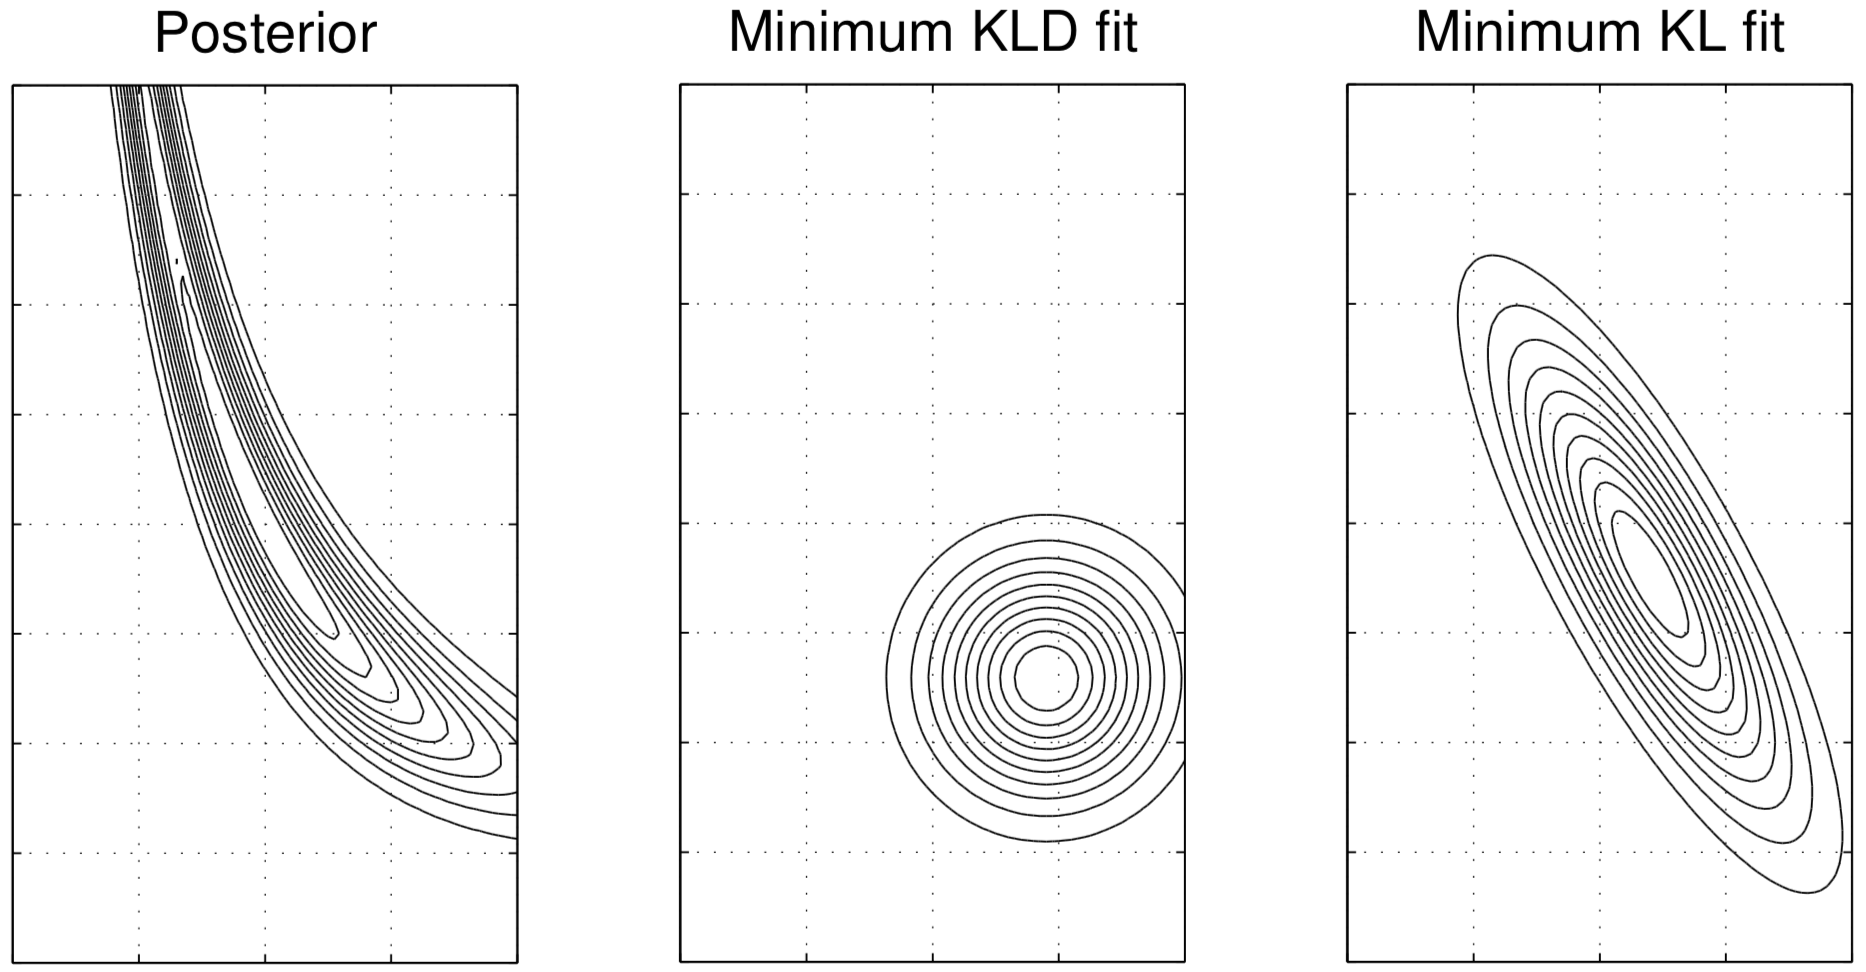
\includegraphics[width=0.7\textwidth]{approximations}
 \label{figure:family}
\end{center}
{Figure 1: Comparison of posterior distribution approximations on a synthetic example with two parameters. A full covariance Gaussian distribution (KL) results in a much improved approximation to the posterior than the diagonal covariance Gaussian distribution (KLD), with a lower residual KL value and better KL fit. `More flexible distributions \textelp{} simply give better approximations to the true posterior'.
\cite{ensemblelearning}}
%A diagonal covariance Gaussian distribution (KLD) results in KL\textsubscript{res} = 4.6, whereas a full covariance Gaussian distribution (KL) results in an improved KL\textsubscript{res} = 3.9. \cite{ensemblelearning}}.

A tractable algorithm for posterior approximation with a full covariance Gaussian distribution has been demonstrated \cite{ensemblelearning}. %Elaborate?

\end{enumerate}
\newpage
We suggest that an investigation into an improvement to the second criterion may also be promising. Approximate Bayesian inference is typically carried out with either variational or Markov Chain Monte Carlo (MCMC) inference. We also suggest looking into using a MCMC approach instead of a variational approach such as KL minimisation. The secondary aim of the project is therefore to see if using MCMC results in better performance:
\begin{enumerate}
\setcounter{enumi}{1}
\item \textbf{Using a Markov Chain Monte Carlo method for posterior approximation.}

Using a Monte Carlo method to sample from the posterior distribution is the closest we can get to exact Bayesian inference in practice, and is advantageous in that it does not impose assumptions about the shape of the posterior distribution \cite{hinton}.

We expect that Hamiltonian Monte Carlo (HMC) is a promising MCMC method to use for approximate inference. HMC is a principled Hamiltonian dynamics-based MCMC method which has been applied successfully to Bayesian neural networks \cite{bayesianlearning}. It systematically and coherently traverses the state space, avoiding the slow exploration typical of random walk proposals \cite{hmc}. This is particularly useful in high-dimensional spaces, where we must use information about the space geometry for an efficient exploration. Gradient-based algorithms such as HMC tend to be more robust and geometrically ergodic over a larger class of target distributions than non-gradient based algorithms, yielding `stronger guarantees on the validity of the resulting estimators' \cite{conceptual}.
% second-gradient - calculating Hamiltonian is really expensive for high dimensional spaces
% HMC sets cap on size of neural network we can use
\end{enumerate}


\subsection*{Approximate Timeline}

\begin{tabular}{l|l}
\hline
March 	& Write project proposal; review literature\\
April	& Use non-continual BNN to compare diagonal and full model families\\
May		& Continue with comparison; \\
&begin continual learning comparison implementation \\
June 	& Continue with continual learning comparison implementation\\
July	& Continue with continual learning comparison implementation; \\
&begin with Markov Chain Monte Carlo implementation\\
August	& Continue with MCMC implementation\\
September 2 & Hand-in date\\
\hline
\end{tabular}

%\subsection*{Project supervisors' signatures}

%\begin{labeling}{projectsupervisors}
%\vspace*{2.25em}
%\item[S. Farquhar] \rule{5cm}{1pt}
%\vspace*{2.5em}
%\item[Y. Gal] \rule{5cm}{1pt}
%\end{labeling}


 

\newpage
\begin{thebibliography}{8}

\bibitem[Barber \& Bishop, 1998]{ensemblelearning} D. Barber, C. M. Bishop, 1998. \textit{Ensemble Learning in Bayesian Neural Networks}. Neural Networks and Machine Learning, Springer, 215-237. \href{https://www.microsoft.com/en-us/research/wp-content/uploads/2016/02/bishop-ensemble-nato-98.pdf}{Link to paper}

\bibitem[Betancourt, 2017]{conceptual} M. Betancourt, 2017. \textit{A Conceptual Introduction to Hamiltonian Monte Carlo}. \href{https://arxiv.org/abs/1701.02434}{arXiv:1701.02434v2}

\bibitem[Chaudhry et al., 2018]{rw} A. Chaudhry, P. K. Dokania, T. Ajanthan, P. H. S. Torr, 2018. \textit{Riemannian Walk for Incremental Learning: Understanding Forgetting and Intransigence}. \href{https://arxiv.org/abs/1801.10112}{arXiv:1801.10112v3}

\bibitem[Farquhar \& Gal, 2019]{unifying} S. Farquhar, Y. Gal, 2019. \textit{A Unifying Bayesian View of Continual Learning}. \href{https://arxiv.org/abs/1902.06494}{arXiv:1902.06494v1}

\bibitem[Farquhar \& Gal, 2018]{robust} S. Farquhar, Y. Gal, 2018. \textit{Towards Robust Evaluations of Continual Learning}. \href{https://arxiv.org/abs/1805.09733}{arXiv:1805.09733v2}

\bibitem[Hinton \& van Camp, 1993]{hinton} G. E. Hinton, D. van Camp, 1993. \textit{Keeping the
Neural Networks Simple by Minimizing Description Length of the Weights}. \href{http://www.cs.toronto.edu/~fritz/absps/colt93.pdf}{Link to paper}

\bibitem[Kirkpatrick et al., 2017]{ewc} J. Kirkpatrick, R. Pascanua, N. Rabinowitza, J. Venessa, G. Desjardinsa, A. A. Rusua, K. Milana, J. Quana, T. Ramalhoa, A. Grabska-Barwinskaa, D. Hassabisa, C. Clopathb, D. Kumarana, and R. Hadsella, 2017. \textit{Overcoming catastrophic forgetting in neural networks}. \href{https://arxiv.org/abs/1612.00796}{arXiv:1612.00796v2}

%\bibitem[MacKay, 1992]{mackay} D. J. C. MacKay, 1992. \textit{A Practical Bayesian Framework for Backpropagation Newtorks}. \href{https://authors.library.caltech.edu/13793/1/MACnc92b.pdf}{Link to paper}

\bibitem[McCloskey \& Cohen, 1989]{catastrophic} M. McCloskey, N. J. Cohen, 1989. \textit{Catastrophic Interference in Connectionist Networks: The Sequential Learning Problem}. Psychology of Learning and Motivation, Volume 24, 109-165.

\bibitem[Neal, 2012]{hmc} R. M. Neal, 2012. \textit{MCMC using Hamiltonian dynamics}. \href{https://arxiv.org/abs/1206.1901}{arXiv:1206.1901v1}

\bibitem[Neal, 1995]{bayesianlearning} R. M. Neal, 1995. \textit{Bayesian Learning for Neural Networks}. \href{http://citeseerx.ist.psu.edu/viewdoc/download?doi=10.1.1.446.9306&rep=rep1&type=pdf}{Link to paper}

\bibitem[Nguyen et al., 2017]{vcl} C. V. Nguyen, Y. Li, T. D. Bui, R. E. Turner, 2017. \textit{Variational Continual Learning}. \href{https://arxiv.org/abs/1710.10628}{arXiv:1710.10628v3}

%\bibitem[Ratcliff, 1990]{connectionist} R. Ratcliff, 1990. \textit{Connectionist Models of Recognition Memory: Constraints Imposed by Learning and Forgetting Functions}. Psychological Review, Vol.97, No. 2, 285-308.

\bibitem[Ritter et al., 2018]{ritter} H. Ritter, A. Botev, D. Barber, 2018. \textit{Online Structured Laplace Approximations For Overcoming Catastrophic Forgetting}. \href{https://arxiv.org/abs/1805.07810}{arXiv:1805.07810v1}

\bibitem[Robins, 1995]{robins} A. Robins. \textit{Catastrophic forgetting, rehearsal, and pseudorehearsal}. Connection Science: Journal of Neural Computing, Artificial Intelligence and Cognitive Research, Volume 7, 123-146.



\bibitem[Shin et al., 2017]{dgr} H. Shin, J. K. Lee, J. Kim, J. Kim, 2017. \textit{Continual Learning with Deep Generative Replay}. \href{https://arxiv.org/abs/1705.08690}{arXiv:1705.08690v3}

\bibitem[Zenke et al., 2017]{si} F. Zenke, B. Poole, S. Ganguli, 2017. \textit{Continual Learning Through Synaptic Intelligence}. \href{https://arxiv.org/abs/1703.04200}{arXiv:1703.04200v3}
%\bibitem[Liu \& Chen, 1998] J. S. Liu, R. Chen, 1998. \textit{Sequential Monte Carlo Methods for Dynamic Systems}. Journal of the American Statistical Association, Vol. 93, No. 443, pp. 1032-1044.




\end{thebibliography}



\end{document}
